% $Header: /cvsroot/latex-beamer/latex-beamer/solutions/generic-talks/generic-ornate-15min-45min.en.tex,v 1.5 2007/01/28 20:48:23 tantau Exp $

\documentclass[12pt]{beamer}
%\documentclass[12pt,handout]{beamer}

% This file is a solution template for:

% - Giving a talk on some subject.
% - The talk is between 15min and 45min long.
% - Style is ornate.



% Copyright 2004 by Till Tantau <tantau@users.sourceforge.net>.
%
% In principle, this file can be redistributed and/or modified under
% the terms of the GNU Public License, version 2.
%
% However, this file is supposed to be a template to be modified
% for your own needs. For this reason, if you use this file as a
% template and not specifically distribute it as part of a another
% package/program, I grant the extra permission to freely copy and
% modify this file as you see fit and even to delete this copyright
% notice.


\mode<presentation>
{
  \usetheme{default}
  % or ...

  \setbeamercovered{transparent}
  % or whatever (possibly just delete it)
}
\setbeamertemplate{navigation symbols}{}%remove navigation symbols


\usepackage[english]{babel}
% or whatever

\usepackage[latin1]{inputenc}
% or whatever

\usepackage{times}
\usepackage{sansmathfonts}
\usepackage[T1]{fontenc}
% Or whatever. Note that the encoding and the font should match. If T1
% does not look nice, try deleting the line with the fontenc.


\title%[Short Paper Title] % (optional, use only with long paper titles)
{}

\subtitle
{} % (optional)

\author%[Author, Another] (optional, use only with lots of authors)
{Ben Holder}%{F.~Author\inst{1} \and S.~Another\inst{2}}
% - Use the \inst{?} command only if the authors have different
%   affiliation.

%\institute[Universities of Somewhere and Elsewhere] % (optional, but mostly needed)
%{
%  \inst{1}%
%  Department of Computer Science\\
%  University of Somewhere
%  \and
%  \inst{2}%
%  Department of Theoretical Philosophy\\
%  University of Elsewhere}
%% - Use the \inst command only if there are several affiliations.
%% - Keep it simple, no one is interested in your street address.

\date%[Short Occasion] % (optional)
{}

\subject{Talks}
% This is only inserted into the PDF information catalog. Can be left
% out.



% If you have a file called "university-logo-filename.xxx", where xxx
% is a graphic format that can be processed by latex or pdflatex,
% resp., then you can add a logo as follows:

% \pgfdeclareimage[height=0.5cm]{university-logo}{university-logo-filename}
% \logo{\pgfuseimage{university-logo}}



% Delete this, if you do not want the table of contents to pop up at
% the beginning of each subsection:
%\AtBeginSubsection[]
%{
%  \begin{frame}<beamer>{Outline}
%    \tableofcontents[currentsection,currentsubsection]
%  \end{frame}
%}


% If you wish to uncover everything in a step-wise fashion, uncomment
% the following command:

%\beamerdefaultoverlayspecification{<+->}

\usepackage{enumerate}
\usepackage{amsmath}
\usepackage{amssymb}
\usepackage[amssymb]{SIunits}
\usepackage{url}
\usepackage{hyperref}
\usepackage[normalem]{ulem}


\setbeamercovered{invisible}

\hypersetup{
    colorlinks=true,     % false: boxed links; true: colored links
    linkcolor=red,       % color of internal links
    citecolor=blue,      % color of links to bibliography
    filecolor=blue,      % color of file links
    urlcolor=blue        % color of external links
}


\begin{document}

%\begin{frame}
%  \titlepage
%\end{frame}

%%%%%%%%%%%%%%%%%%%%%%%%%%%%%%%%%%%%%%
\begin{frame}{Announcements}
	%
	\begin{itemize}
	\addtolength{\itemsep}{0.5\baselineskip}
	\item Everyone getting their marked-up things back?
	\item Assignment turn-in and Grading (next slide)
	\item \underline{Schedule}:
		%
		\begin{itemize}
		\item[]{\bf Today (Lecture)}: Newton's Laws, Energy, Energy Transfer, Equilibrium
		\item[]{\bf Tomorrow (Lab)}: Motion, Energy, and Equilibrium
		\item[]{\bf Thursday (Discussion)}]: Analyzing Enegy Transfer
		\item Next Week: Electromagnetic Radiation (Light) and Blackbody Radiation
		\end{itemize}
		%
	\end{itemize}

\end{frame}
%%%%%%%%%%%%%%%%%%%%%%%%%%%%%%%%%%%%%%
\begin{frame}{Assignments: Turn-In and Grading}
	%
	\begin{itemize}
	\addtolength{\itemsep}{0.5\baselineskip}
	\item Each assignment turned in as \underline{single PDF} document
	\item Prepare as if you were going to turn in a hard copy, then scan with {\em Adobe Scan} app. Ask me for help!
	\end{itemize}
	
	\underline{Labs}: Turn in:
		%
		\begin{itemize}
		\item all pages with answers, measurements, calculations, etc; 
		\item all data sets produced by hand (large downloaded ones not necessary)
		\item all plots/graphs produced
		\end{itemize}
	\underline{Grading} for assignments
		%
		\begin{itemize}
		\item[]{\bf C} $\approx$ 75: You turned it in, mostly complete
		\item[]{\bf B} $\approx$ 85: You demonstrated effort, majority correct
		\item[]{\bf A} $\approx$ 95: You demonstrated careful effort, thought, and logic; clearly discussed issues with partners and me;  mostly correct
		\end{itemize}
		%

\end{frame}
%%%%%%%%%%%%%%%%%%%%%%%%%%%%%%%%%%%%%%
\begin{frame}{Today's Reading Quiz (3 min)}

\underline{Grading} for reading quizzes:
	\begin{itemize}
	\item[] {\bf 80}: You turned it in
	\item[] {\bf 90}: You demonstrated that you read, have basic ideas
	\item[] {\bf 100}: Correct answer, demonstrated you internalized ideas (or took careful notes)	
	\end{itemize}
	
\vspace{1cm}

On your own sheet of paper\ldots

\vspace{0.5cm}

{\bf What does it mean for an object/system to be in equilibrium? How does it relate to ``energy in'' and ``energy out''? What is true about the internal state of the system when in equilibrium?}

\vspace{0.5cm}

Turn in to Blackboard as scanned pdf (or image is fine).

\end{frame}
%%%%%%%%%%%%%%%%%%%%%%%%%%%%%%%%%%%%%%
\begin{frame}{Today: Energy and Equlibrium}

{\tiny (AKA: Most of first-semester introductory physics in 40 minutes!)}
\vfill

Why are we doing this?
\begin{itemize}
\item Last week: temperature of the Earth is increasing.
\item Also: (circumstantial) evidence that $\text{CO}_2$ is responsible
\item So \ldots why do we need more?
\end{itemize}

A careful {\em physical} explanation/description will:
\begin{itemize}
\item allow us to understand the mechanism for the change, 
\item give more solid evidence for {\em attribution} of climate change, 
\item provide \underline{models} to predict the future
\end{itemize}

\hspace{1.5cm} %
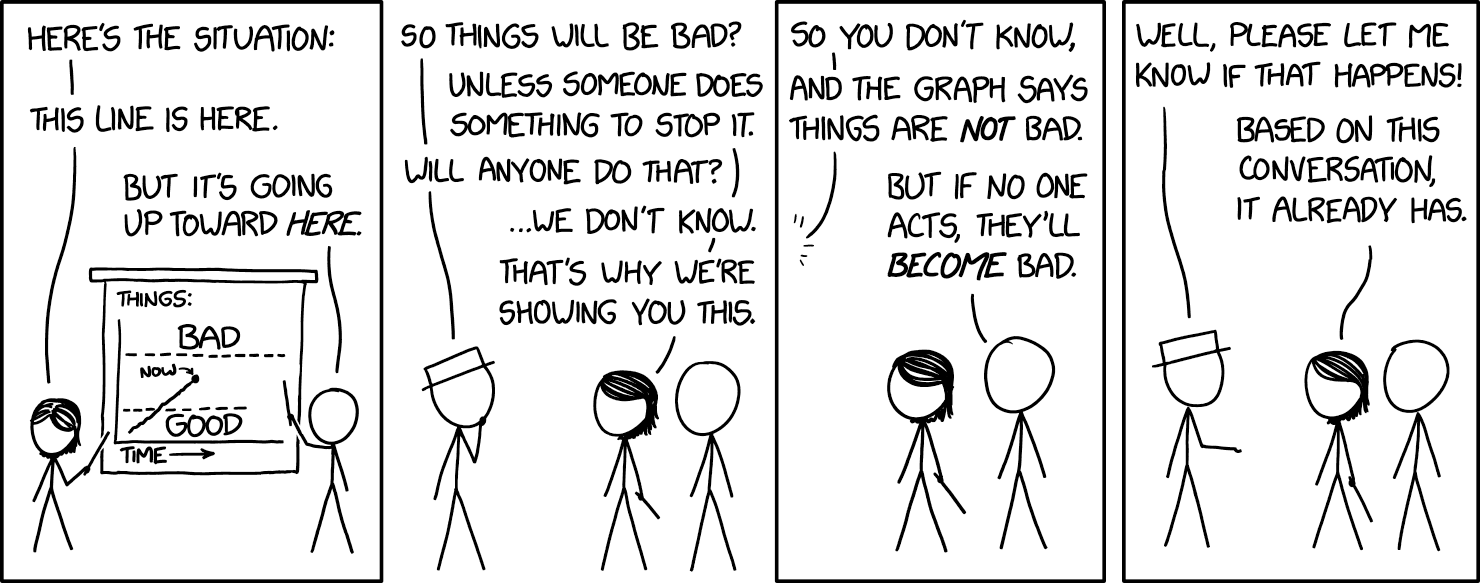
\includegraphics[width=0.7\textwidth]{images/xkcd_scientific_briefing_2x.png}

\end{frame}
%%%%%%%%%%%%%%%%%%%%%%%%%%%%%%%%%%%%%%
\begin{frame}{Motion}

We describe the motion an object using three quantities:
	%
	\begin{itemize}
	\item[] {\bf Position}, $x$: Where is the object?
	\item[] {\bf Velocity}, $v$: How fast is it ``going''? ($\Delta x / \Delta t$)
	\item[] {\bf Acceleration}, $a$: How is the velocity changing?  ($\Delta v / \Delta t$)
	\end{itemize}
	%
Each of these has a {\em direction} associated, so sometimes they are expressed as {\em vectors}, e.g., $\vec{v}$, $\vec{a}$.

\vspace{0.25cm}

\underline{2D Motion (track from above)} \hfill \underline{1D Motion (on ``$x$'' axis)}

\vspace{3.5cm}

What is the (average) speed of a car going from GR to Detroit (140 miles) in 2h30m?

\end{frame}
%%%%%%%%%%%%%%%%%%%%%%%%%%%%%%%%%%%%%%
\begin{frame}{First type of Energy: Kinetic Energy}

We say that a moving object has {\em kinetic energy}:
	%
	\begin{equation*}
	\text{Kinetic Energy} = K = \frac{1}{2} m v^2
	\end{equation*}
	%
where $m$ is the mass and $v$ is the speed.

\vspace{0.5cm}

\underline{Cars (1000 kg) and Trucks (50,000 kg) on the highway}

\vspace{3.5cm}

How much faster would a car have to drive to have same $K$?

\end{frame}
%%%%%%%%%%%%%%%%%%%%%%%%%%%%%%%%%%%%%%
\begin{frame}{Old (wrong) Law of Motion}

\underline{Aristotle (350 BCE)}: {\bf What makes it go?}
	%
	\begin{itemize}
	\item Objects are naturally at rest
	\item A ``violent external agent'' is needed to make them move
	\item Once the violent agent stops, the motion ceases
	\end{itemize}
	%
\underline{Try pushing a box:}

\vspace{4cm}

``Makes sense'' \ldots but the question (and answer) are wrong!

\end{frame}
%%%%%%%%%%%%%%%%%%%%%%%%%%%%%%%%%%%%%%
\begin{frame}{\underline{The} Law of Motion: ``Newton's Second Law''}

\underline{Newton (1687)}: {\bf What makes it {\em change} its motion?}
	%
	\begin{equation*}
	\text{Sum of Forces} = \text{mass} \times \text{acceleration} \quad \rightarrow \quad \vec{a} = \frac{\sum \vec{F}}{m}
	\end{equation*}
	%
So: {\em accelerations} (changes in velocity) are caused by forces (Aristotle's ``violent'' actions)

\vspace{0.25cm}

\underline{Same ``pushing the box'' experiment, but on ice:}

\vspace{4cm}

\end{frame}
%%%%%%%%%%%%%%%%%%%%%%%%%%%%%%%%%%%%%%
\begin{frame}{Graphs of Motion (position and velocity vs time)}

\underline{Three cases are demonstrated}:\\
(i) car at rest; (ii) car pushed and stopped; (iii) car on hill

\vspace{7cm}

When does {\em acceleration} happen?  {\em Why} does it happen?
\end{frame}
%%%%%%%%%%%%%%%%%%%%%%%%%%%%%%%%%%%%%%
\begin{frame}{Other motion concepts (demonstrated)}

\begin{itemize}
\item Effect of increasing object mass with same applied force.
\item Newton's Third Law: Equal but opposite forces in any interaction.
\end{itemize}


\end{frame}
%%%%%%%%%%%%%%%%%%%%%%%%%%%%%%%%%%%%%%
\begin{frame}{Back to Energy... ``Work''}

The concept of energy starts with:
	%
	\begin{center}
	{\em Work done by a force gives energy to an object}
	\end{center}
	%
which is defined as:
	%
	\begin{equation*}
	\text{Work} = \text{Force} \times \text{Distance Applied}
	\end{equation*}
	
\vspace{0.25cm}

\underline{Pushing the box, on ice or not:}

\vspace{4cm}

Work on the box increases its kinetic energy: $ W = \Delta K$.

\end{frame}
%%%%%%%%%%%%%%%%%%%%%%%%%%%%%%%%%%%%%%
\begin{frame}{Potential Energy}

So far we have: 
	%
	\begin{itemize}
	\item Kinetic energy (of motion)
	\item Work: Transfer of energy by a force
	\end{itemize}
	%
Now a second type of energy: {\em Potential Energy}

\vspace{0.15cm}

\underline{Springs}

\vspace{2cm}

\underline{Gravity}

\vspace{2cm}

Systems like this can ``hold'' energy. They have the {\em potential to do work} with their forces.

\end{frame}
%%%%%%%%%%%%%%%%%%%%%%%%%%%%%%%%%%%%%%
\begin{frame}{Conservation of Energy (I --- Mechanical)}

From Newton's Laws, one can derive the principle of \underline{energy conservation}:
	%
	\begin{quote}
	\textit{In a closed mechanical system, energy can be transferred from kinetic to potential, but never lost/destroyed.}
	\end{quote}
	%

\underline{Example with block, spring, hill:}
	
\vspace{6cm}

\end{frame}
%%%%%%%%%%%%%%%%%%%%%%%%%%%%%%%%%%%%%%
\begin{frame}{Another type of energy transfer: Heat}

Aristotle's box (not on ice) stopped because:
	%
	\begin{itemize}
	\item There is a {\em frictional} force opposing the motion
	\item Work done by that frictional force takes energy out of motion, {\em heating} the block and the surface.
	\end{itemize}
	%
So we now have a second mechanism (in addition to work) of energy transfer: \underline{Heat}

\vspace{6cm}

\end{frame}
%%%%%%%%%%%%%%%%%%%%%%%%%%%%%%%%%%%%%%
\begin{frame}{Internal Energy (Solids)}

Where does energy lost to friction go?  What does it mean that the block and surface get ``heated''?

\vspace{0.25cm}

We can think of solid objects as huge collections of masses connected by springs (these are actually atoms, with chemical/quantum bonds).  Frictional-type forces do work on the little particles on the surface --- causing spring compression (potential energy) and vibration (kinetic energy) --- which then transfers into motion of internal particles.

\vspace{6cm}

\end{frame}
%%%%%%%%%%%%%%%%%%%%%%%%%%%%%%%%%%%%%%
\begin{frame}{Internal Energy (Fluids)}

For a gas or liquid, the internal energy is simply the sum of the kinetic energy of the particles.



\vspace{6cm}

{\em Temperature} is a measure of the average kinetic energy of such a system.  

\end{frame}
%%%%%%%%%%%%%%%%%%%%%%%%%%%%%%%%%%%%%%
\begin{frame}{Energy Types (Summary)}

\begin{itemize}
\item Kinetic
\item Potential
\item Internal (kinetic and potential)
\item Chemical (bonds)
\item Electrical 
\item Nuclear
\end{itemize}

\end{frame}
%%%%%%%%%%%%%%%%%%%%%%%%%%%%%%%%%%%%%%
\begin{frame}{Energy Transfer Types (Summary)}

\begin{itemize}
\item Work (by force)
\item Heating (or conduction)
\item Convection 
\item Radiation
\end{itemize}

\end{frame}
%%%%%%%%%%%%%%%%%%%%%%%%%%%%%%%%%%%%%%
\begin{frame}{Energy Transfer Diagrams/Analysis}


\end{frame}
%%%%%%%%%%%%%%%%%%%%%%%%%%%%%%%%%%%%%%
\end{document}
